


\begin{document}

This section details the experimental implementation of the two differential amplifiers, the resistively loaded and active loaded. The power supplies and analysis were implemented using the Digilent Analog Discovery kit. The experimental circuit can be seen Figure \ref{fig:expercircuit}.

\begin{figure}[H]
	\begin{center}
		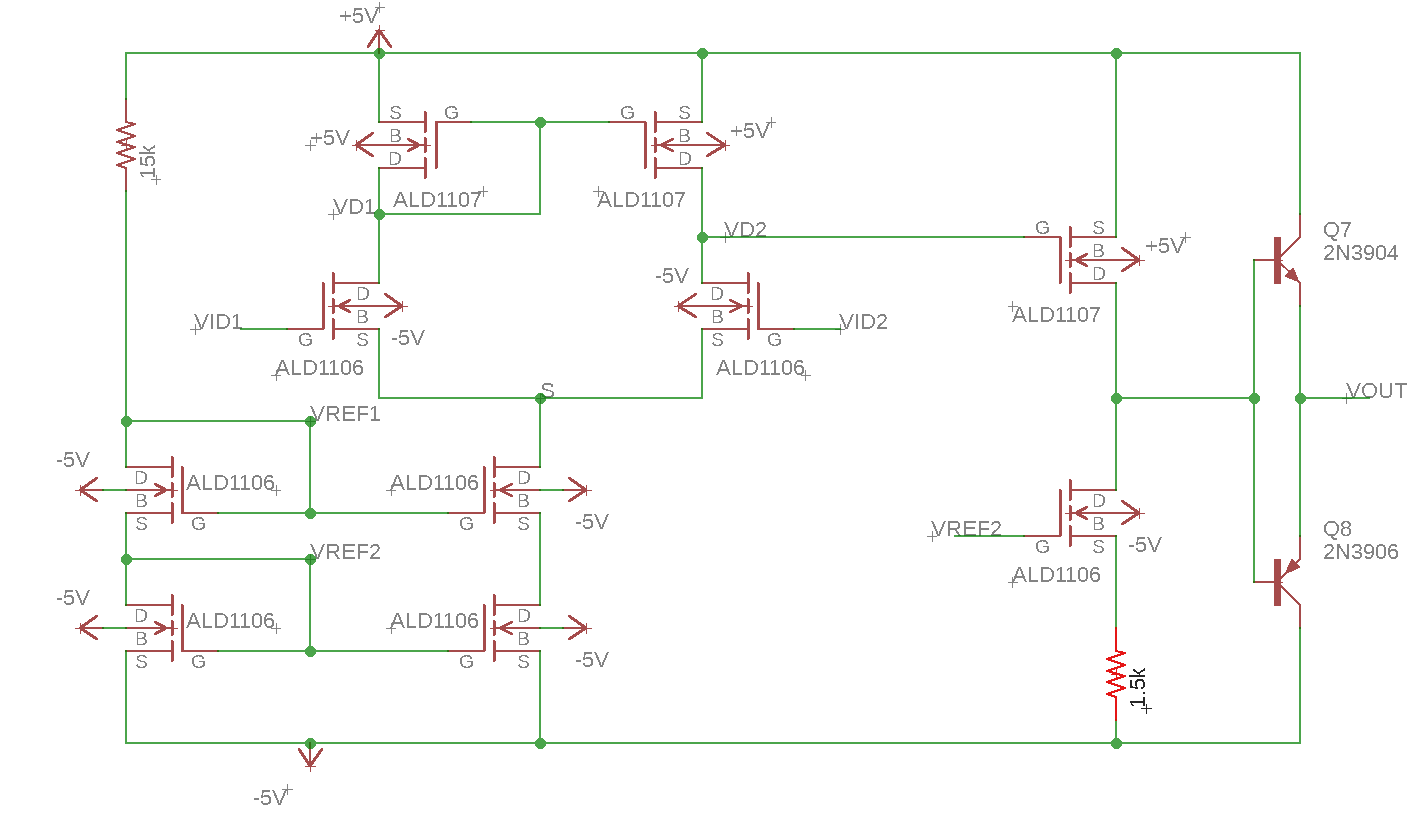
\includegraphics[scale=.40]{ExperimentalImplementation/final_schem.png}
		\caption{Experimental operational amplifier}
		\label{fig:expercircuit}
	\end{center}
\end{figure}
The simulated circuit, when constructed, failed to meet both the final differential gain output of 46 dB as well as the CMRR of 60 dB. As a result the final circuit design was changed to the op amp design \#1, which can be seen in Figure \ref{fig:expercircuit}. Further details on why design was changed can be found in the Discussion section.

The DC bias conditions were measured using a DT830B DVM. Nodal voltages were measured in reference to ground and current was measured by wiring the DVM in series while in ammeter mode. The bias conditions were measured while both input nodes to the circuit were grounded. The final measured values can be seen in Table \ref{tab:expdc}.


\begin{table}[H]
	\centering
	\caption{Experimental DC values}
	\label{tab:expdc}
	\begin{tabular}{|l|l|}
		\hline
		\textbf{DC Bias Conditions} &           \\ \hline
		Vref                        & -2.97V    \\ \hline
		Iref                        & 396$\mu$A \\ \hline
		D1                          & 2.01V     \\ \hline
		D2                          & 1.99V     \\ \hline
		S                           & -2.04V    \\ \hline
		OutCS                       & 100mV      \\ \hline
	\end{tabular}
\end{table}

Notably, the voltage at the "OutCS" node should be zero. In the default state, the offset at that node was measured to be 2.5V. A potentiometer was used as the source degeneration resistance for the common source amplifier. This pot was varied until the offset was nulled out and the final resistance value required was found to be 1.5k$\Omega$. The range of operation for the circuit can be seen in Figure \ref{fig:vtc}.


\begin{figure}[H]
	\begin{center}
		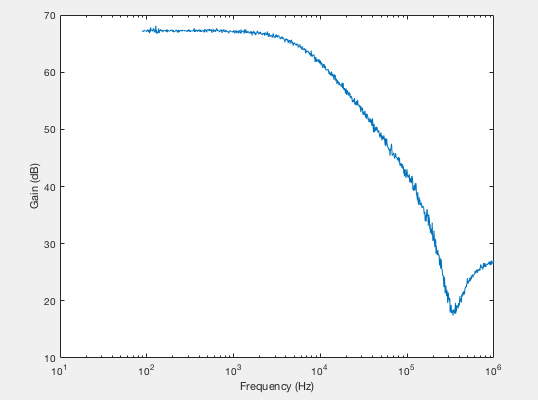
\includegraphics[scale=.40]{ExperimentalImplementation/Ad_final.png}
		\caption{Experimental range of operation}
		\label{fig:vtc}
	\end{center}
\end{figure}

The range of operation is extremely narrow. This, however, is expected due to the limits imposed by the use of a cascode current mirror. The cascode affords more gain at the expense of voltage range. This was explored in more depth in Task 3. In order to prevent the op amp from saturating, a 1000:1 voltage divider was added at the signal input. The channel 1 probe was connected after the voltage divider to compensate for the 60dB drop from the voltage divider. Channel 2 was connected at the final output of the operational amplifier. The final differential gain can be seen in Figure \ref{fig:finalAD}.

\begin{figure}[H]
	\begin{center}
		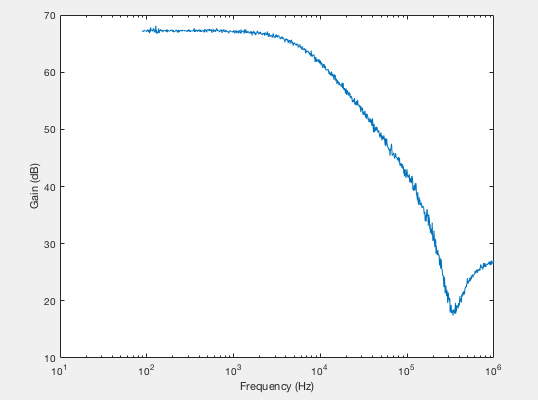
\includegraphics[scale=.40]{ExperimentalImplementation/Ad_final.png}
		\caption{Experimental differential gain}
		\label{fig:finalAD}
	\end{center}
\end{figure}

The max differential gain can be seen to be 67 dB. This is more than 20 dB greater than the minimum specification. Even more noteworthy, however, is the fact that the gain is not unity gain stable. The gain plot, at least within the range of 100 Hz to 1MHz, never crosses the 0 dB point. As a result, the amplifier is said to not be unity gain stable. This can be remedied by including a capacitor at the output stage and will be done during Task 5. The phase of the differential gain phase can be seen in Figure \ref{fig:adphase}. 

\begin{figure}[H]
	\begin{center}
		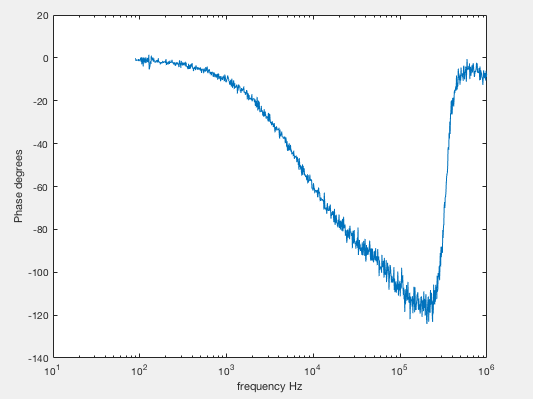
\includegraphics[scale=.40]{ExperimentalImplementation/Ad_phase.png}
		\caption{Experimental differential gain phase}
		\label{fig:adphase}
	\end{center}
\end{figure}

The phase can be seen to return to unity after 100kHz. This is also a result of the lack of frequency compensation. Notably, the phase mirrored that of the simulated design quite well. The final design spec is that the circuit must achieve a CMRR of at least 60 dB. In order to find the CMRR the common mode gain must be found by applying a signal to both inputs while measuring the output gain via the Analog Discoveries Network analyzer mode. The common mode gain for both 100mV and 1V can be seen in Figure \ref{fig:acmexp}.


\begin{figure}[H]
	\centering
	\begin{subfigure}[b]{0.45\textwidth}
		\centering
		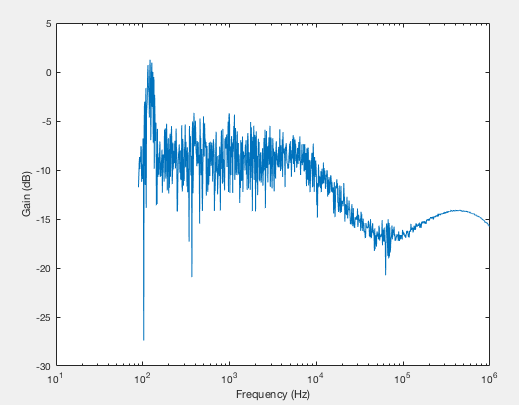
\includegraphics[width=\textwidth]{ExperimentalImplementation/Acm_100mv.png}
		\caption{Common mode gain, Acm at 100mV}
		\label{fig:blue_led}
	\end{subfigure}
	\hfill
	\begin{subfigure}[b]{0.45\textwidth}
		\centering
		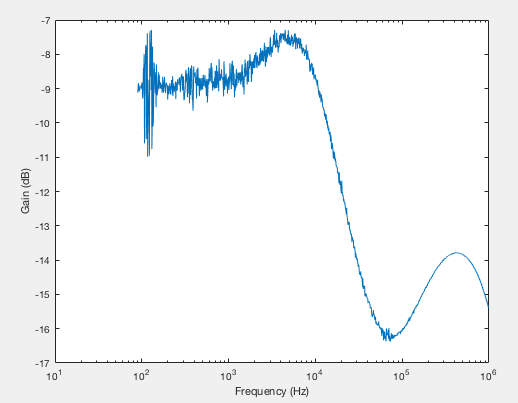
\includegraphics[width=\textwidth]{ExperimentalImplementation/Acm_1v.png}
		\caption{Acm, single ended}
		\label{fig:blue_led}
	\end{subfigure}
	\caption{Common mode gain, Acm at 1V}
	\label{fig:acmexp}
\end{figure} 

The common mode gain is still negative, which is desired. The Acm is -10dB this is, however, much lower than what was found in Task 3, which was found to be on the order of -60 dB. This is mostly due to the fact that a significant portion of the op amps gain is now coming from the common source stage and not just the active load differential pair. The CMRR is then found by finding the difference between the differential gain and the common mode gain in Matlab.


\begin{figure}[H]
	\begin{center}
		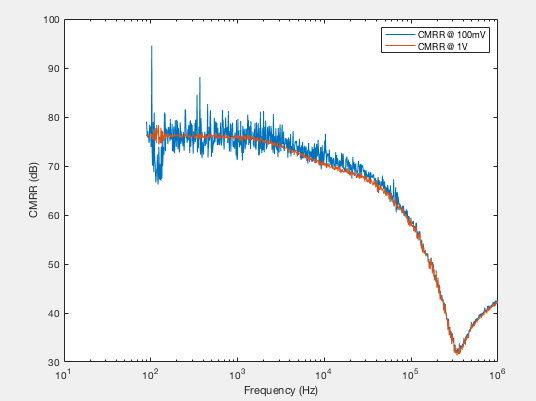
\includegraphics[scale=.40]{ExperimentalImplementation/CMRR_fin.png}
		\caption{Experimental common mode rejection ratio}
		\label{fig:cmrr}
	\end{center}
\end{figure}

 As expected, the CMRR was much cleaner when the input signal was 1V as opposed to a 100mV signal. The measured value was 75 dB, which is greater than the minimum specification of 60 dB. The summary of experimental values can be seen in Table \ref{tab:expfin}.
 
 
 \begin{table}[H]
 	\centering
 	\caption{Final experimental values}
 	\label{tab:expfin}
 	\begin{tabular}{|l|l|}
 		\hline
 		\textbf{Experimental Values} &       \\ \hline
 		Ad                           & 67dB  \\ \hline
 		Acm                          & -10dB \\ \hline
 		CMRR                         & 75 dB \\ \hline
 	\end{tabular}
 \end{table}

The experimental values all met specifications. Further discussion of the op amp and why the changes were made between the design's can be found in the Discussion section.


 
\end{document}


